
\section{作用量泛函莫尔斯理论的 Floer 方法}
\label{sec:floer-morse}

\hzsync{theorem}{10}%
\hzsync{proposition}{12}%
\hzsync{equation}{112}%

我们将勾画\trFloer{}求解\trArnold{}猜想的那个开创性进路，它处理的是非退化%
情形：即假设 $(M,\omega)$ 上\trHamiltonianSystem{}的全体 $1$-\trPeriodicSolution%
都\trNondegenerate。由于 $M$ \trCompact，这样的 $1$-\trPeriodicSolution{}只有%
有限多个。\trFloer{}研究了由\trActionFunctional{}在 $M$ 的可缩\trLoop{}之空间上%
定义的未\trRegularization{}的\trGradient{}方程之\trBounded\trOrbit{}集。这些%
有界\trOrbit{}是某一特定的\trCauchy-\trRiemann{}型一阶椭圆方程组的特殊解，%
如我们上文所证明的。但与上一节所研究的一般情形不同，在非退化情形，诸有界%
\trOrbit{}在一种强意义下渐近地趋于\trHamiltonianEquation{}的诸%
$1$-\trPeriodicSolution。\trFloer{}利用解集合的这一附加结构，借助\trFredholm{}%
理论构造了一个由这有限多个 $1$-\trPeriodicSolution{}生成的%
\textbf{\trChainComplex}（chain complex）。该复形的同调称为\textbf{\trFloer{}%
同调}（Floer homology）；它是底\trManifold{}的一个\trInvariant{}量。通过把该%
复形\trContinuation{}到由 $M$ 上\trHamiltonianFunction{}的\trGradient{}系统%
$\dot{y}=-\nabla H(y)$ 所定义的经典\textbf{\trMorse{}复形}（Morse complex），%
\trFloer{}最终证明了他的同调是\trManifold{}的\textbf{\trSingularHomology}%
（singular homology）的一个模型。这样就完成了\trArnold{}猜想的证明。

我们考虑一个维数为 $2n$ 的\trCompact\trSymplecticManifold{} $(M,\omega)$，它%
受要求 $[\omega]\big|_{\pi_{2}(M)}=0$ 的限制。这意味着\trSymplecticStructure{}%
在每张球面上的\trIntegral{}都为零
\begin{equation}\label{eq:floer-omega-spheres}
\int_{S^{2}}u^{*}\omega\ =\ 0\,,\qquad u:S^{2}\to M\,.
\end{equation}
对一个\trSmooth{}的\trTimeDependent\trHamiltonianFunction{}%
$H:S^{1}\times M\to\R$——它关于时间\trPeriodic，即对 $t\in\R$ 与 $x\in M$ 有%
$H(t,x)=H(t+1,x)$——我们像通常那样借 $\omega(X_{H},\cdot)=-d_{x}H(t,x)$ 配以%
\trHamiltonianVectorField{} $X_{H}:\R\times M\to TM$。\trTimeDependent%
\trHamiltonianEquation
\begin{equation}\label{eq:floer-ham-eq}
\dot{x}(t)\ =\ X_{H}\Bigl(t,x(t)\Bigr)\quad\text{于 }M
\end{equation}
的解 $x(t)$ 定义了\trFlow{} $\psi^{t}$：$\psi^{t}(x(0))=x(t)$。我们要找的是%
\trPeriodicSolution{} $x(t+1)=x(t)$，它们是 $M$ 上的可缩\trLoop，$x\simeq0$。%
我们将假设全体可缩\trPeriodicSolution{} $x(t)$ 都\trNondegenerate，这要求%
\trFlow{}映射 $\psi=\psi^{1}$ 满足
\begin{equation}\label{eq:floer-nondegen}
\det\Bigl(1-d\psi\bigl(x(0)\bigr)\Bigr)\ \neq\ 0\,.
\end{equation}
以 $\mathcal{P}_{H}$ 表示这些\trPeriodicSolution{}之集：
\begin{equation}\label{eq:floer-PH}
\begin{aligned}
\mathcal{P}_{H}\ =\ \Bigl\{\,x:S^{1}\to M\ \Bigm|\ &x(t+1)=x(t)\,,\ x\ \text{满足}\ \eqref{eq:floer-ham-eq}\ \text{与}\ \eqref{eq:floer-nondegen}\,,\\
&\text{且}\ x\simeq0\,\Bigr\}\,.
\end{aligned}
\end{equation}
注意这是一个有限集，因为 $M$ \trCompact{}而\trNondegenerate{}的%
$1$-\trPeriodicSolution{}在 $M$ 中孤立。以 $\Omega$ 表示 $M$ 的\trSmooth{}可缩%
\trLoop{} $\gamma$ 之集，此处照例 $S^{1}=\R/\Z$。一条\trLoop{}可提升为满足%
$\gamma(t+1)=\gamma(t)$ 的映射 $\gamma:\R\to M$（周期延拓）。所求的诸%
$1$-\trPeriodicSolution{}在 $\Omega$ 中作为\trActionFunctional{}%
$\varphi_{H}:\Omega\to\R$ 的诸\trCriticalPoint{}而被挑出，$\varphi_{H}$ 定义为
\begin{equation}\label{eq:floer-action}
\varphi_{H}(\gamma)\ =\ -\int_{D}\bar{\gamma}^{\,*}\omega\ +\ \int_{0}^{1}H\Bigl(t,\gamma(t)\Bigr)\,dt\,.
\end{equation}
此处 $D\subset\C$ 表示闭单位\trDisc，而 $\bar{\gamma}:D\to M$ 是延拓 $\gamma$%
的一个\trSmooth{}函数，从而满足 $\bar{\gamma}(e^{2\pi it})=\gamma(t)$。这样的%
延拓存在，因为 $\gamma$ 被假设为可缩；而由假设%
\eqref{eq:floer-omega-spheres} 可知，\eqref{eq:floer-action} 右端第一个%
\trIntegral{}不依赖于延拓的选取，因而只依赖于\trLoop{} $\gamma$。以%
$T_{\gamma}\Omega$ 表示在 $\gamma\in\Omega$ 处的切空间，它由沿 $\gamma$ 的%
\trSmooth{}\trVectorField{} $\xi\in C^{\infty}(\gamma^{*}TM)$ 组成，满足%
$\xi(t+1)=\xi(t)$。沿方向 $\xi$ 计算 $\varphi_{H}$ 的\trDerivative，容易发现
\begin{equation}\label{eq:floer-dphi}
d\varphi_{H}(\gamma)\xi\ =\ \int_{0}^{1}\bigl\{\omega(\dot{\gamma},\xi)\ +\ dH(t,\gamma)\xi\,\bigr\}\,dt\,,
\end{equation}
的确，它对每个 $\xi\in T_{\gamma}\Omega$ 为零当且仅当\trLoop{} $\gamma\in\Omega$%
是\trHamiltonianEquation{} \eqref{eq:floer-ham-eq} 的一个解。为方便起见，选取%
$M$ 上一个与 $\omega$ \trCompatible{}的\trAlmostComplexStructure{} $J$（见%
第 1 章）。这是一个自同态 $J\in C^{\infty}(\operatorname{End}TM)$，即%
$J_{x}\in L(T_{x}M,T_{x}M)$ 满足 $J^{2}=-1$，使得
\begin{equation}\label{eq:floer-metric-g}
g(\xi,\eta)\ =\ \omega\Bigl(\xi,J(x)\eta\Bigr)\,,\qquad \xi,\eta\in T_{x}M
\end{equation}
定义了 $M$ 上的一个\trRiemann{}度量 $g$。于是\trHamiltonianVectorField{}表示为
\begin{equation}\label{eq:floer-XH-Jgrad}
X_{H}(t,x)\ =\ J(x)\nabla H(t,x)\,,
\end{equation}
其中 $\nabla$ 表示 $M$ 上的函数关于 $x$ 变量在上述度量 $g$ 下的\trGradient。%
对其\trDerivative{}我们得到
\begin{equation}\label{eq:floer-dphi-g}
d\varphi_{H}(\gamma)\xi\ =\ \int_{0}^{1}g\Bigl(J(\gamma)\dot{\gamma}\ +\ \nabla H(t,\gamma),\xi\Bigr)\,dt\,,
\end{equation}
于是 $\varphi_{H}$ 关于 $\Omega$ 上一个诱导的 $L^{2}$ 度量的\trGradient{}为
\begin{equation}\label{eq:floer-grad-phi}
\operatorname{grad}\,\varphi_{H}(\gamma)\ =\ J(\gamma)\dot{\gamma}\ +\ \nabla H(\gamma)\ \in\ T_{\gamma}\Omega\,.
\end{equation}
然而，\trGradient{}方程
\begin{equation}\label{eq:floer-grad-eq}
\frac{d}{ds}\,x\ =\ -\ \operatorname{grad}\,\varphi_{H}(x)\,,\qquad x\in\Omega
\end{equation}
不确定一个\trFlow。正如我们在上一节所指出的，由于导数的损失，不存在任何%
\trBanach{}空间框架能把 $\operatorname{grad}\varphi_{H}(x)$ 视为某个\trBanach{}%
流形上的\trVectorField。的确，由 \eqref{eq:floer-grad-eq} 在 $\Omega$ 上定义的%
\trCauchy\trInitialValueProblem{}是不适定的。\trFloer{}把 \eqref{eq:floer-grad-eq}%
的解 $x$ 视为映射
\begin{equation}\label{eq:floer-u-map}
u\ :\ \R\times S^{1}\ \longrightarrow\ M\,,\qquad (s,t)\ \mapsto\ u(s,t)\ =\ u(s,t+1)
\end{equation}
它求解偏微分方程
\begin{equation}\label{eq:floer-pde}
\frac{\partial u}{\partial s}\ +\ J(u)\frac{\partial u}{\partial t}\ +\ \nabla H(t,u)\ =\ 0\,.
\end{equation}

从现在起至关紧要的对象，因而是非线性偏微分方程 \eqref{eq:floer-pde} 的那些%
可缩解 $u:\R\times S^{1}\to M$，可缩使得 $u(s,\cdot)\in\Omega$。这些解对应于%
\trGradient{}方程 \eqref{eq:floer-grad-eq} 的\trFlow{}线。方程%
\eqref{eq:floer-pde} 是一个\trCauchy-\trRiemann{}方程的\trPerturbation。%
\trSmooth{}映射 $u:S^{2}\to M$ 若求解\trCauchy-\trRiemann{}方程
\begin{equation}\label{eq:floer-holo-sphere}
\frac{\partial u}{\partial s}\ +\ J(u)\frac{\partial u}{\partial t}\ =\ 0
\end{equation}
则称为一张\trHolomorphic{}球面。它满足
\begin{equation}\label{eq:floer-sphere-area}
\int_{S^{2}}u^{*}\omega\ =\ \frac{1}{2}\int_{S^{2}}\bigl|\nabla u\bigr|^{2}\,,
\end{equation}
从而我们的假设 \eqref{eq:floer-omega-spheres} 特别排除了非常值的%
\trHolomorphic{}球面。

从\trTorus{}情形我们知道，并非 \eqref{eq:floer-pde} 的所有解都相关，我们只对%
「有界\trOrbit」之集感兴趣，把它记作 $\mathcal{M}\equiv\mathcal{M}(H,J)$。%
这个集定义为这样的\trSmooth{}映射 $u:\R\times S^{1}\to M$ 之集：它们可缩、%
求解方程 \eqref{eq:floer-pde}，此外还具有有限的「能量」
\begin{equation}\label{eq:floer-energy}
E(u)\ :=\ \frac{1}{2}\int_{-\infty}^{\infty}\int_{0}^{1}\Bigl\{\Bigl|\frac{\partial u}{\partial s}\Bigr|^{2}\ +\ \Bigl|\frac{\partial u}{\partial t}-X_{H}(t,u)\Bigr|^{2}\Bigr\}\,ds\,dt\ <\ \infty\,.
\end{equation}
等价地，$\mathcal{M}$ 是可缩解 $u$ 的空间，沿着它们，递减函数%
$\varphi_{H}\bigl(u(s)\bigr)$ 对一切 $s\in\R$ 保持有界，此处%
$u(s)(t)=u(s,t)\in\Omega$。

\trFloer{}在 [85] 中证明：偏微分方程 \eqref{eq:floer-pde} 的\trBounded{}解%
空间 $\mathcal{M}$ 具有一种结构，看上去就像\trSmooth、\trCompact{}且有限维%
\trManifold{}上的一个\trMorse-\trSmale{}系统的结构，下文即来描述。

由于 $M$ \trCompact{}而 $[\omega]$ 依假设 \eqref{eq:floer-omega-spheres} 在%
$\pi_{2}(M)$ 上为零，利用椭圆正则性理论便得出：解集 $\mathcal{M}$ 在「连同%
全部导数于紧集上一致收敛」的\trTopology{}下\trCompact。这并不容易证明，我们%
参考 A.~\trFloer{} [85]、D.~\trSalamon{} [188] 以及 H.~\trHofer{}与%
D.~\trSalamon{} [119]。此外，对每条有界\trOrbit{} $u\in\mathcal{M}$，存在一对%
\trPeriodicSolution{} $x,y\in\mathcal{P}_{H}$，使得 $u$ 是一条从 $y$ 到 $x$ 的%
\trConnectingOrbit，即
\begin{equation}\label{eq:floer-asymptotic}
\lim_{s\to-\infty}u(s,t)\ =\ y(t)\,,\qquad \lim_{s\to+\infty}u(s,t)\ =\ x(t)\,,
\end{equation}
收敛关于 $t$ 一致（当 $|s|\to\infty$），且 $\frac{\partial u}{\partial s}$ 也%
一致地收敛到零。给定两个\trPeriodicSolution{} $x,y\in\mathcal{P}_{H}$，我们%
缩记
\begin{equation}\label{eq:floer-myx}
\mathcal{M}(y,x)\ =\ \mathcal{M}(y,x;H,J)
\end{equation}
为满足渐近边界条件 \eqref{eq:floer-asymptotic} 的解 $u\in\mathcal{M}$ 之集。%
对能量可算得
\begin{equation}\label{eq:floer-energy-myx}
E(u)\ =\ \varphi_{H}(y)-\varphi_{H}(x)\,,\qquad\text{若 }u\in\mathcal{M}(y,x)\,.
\end{equation}
能量对非常值\trOrbit{}为正。从上一节我们知道，解之集 $\mathcal{M}$ 由%
\trPeriodicSolution{}与\trConnectingOrbit{}组成：
\begin{equation}\label{eq:floer-m-union}
\mathcal{M}\ =\ \bigcup_{y,x\in\mathcal{P}_{H}}\mathcal{M}(y,x)\,.
\end{equation}

群 $\R$ 通过沿 $s$ 方向平移 $u(s,t)$ 自然地作用在 $\mathcal{M}$ 上，从而定义%
了空间 $\mathcal{M}$ 上的一个连续\trFlow。在这个作用下，诸集合%
$\mathcal{M}(y,x)$ 是\trInvariant{}子空间。它们的\trCompactness{}可以仿照%
M.~\trSchwarz{}在其专著 [191] 中所表述的有限维\trMorseTheory{}给出类似的表述：

\begin{proposition}\label{prop:broken-orbit-compactness}
\footnote{原书此号与 §6.4 之命题 12 撞号，系原书编号笔误，照实复刻。——译者注}
序列 $u_{\nu}\in\mathcal{M}(y,x)$ 拥有一个具下述性质的子序列：存在时刻的序列%
$s_{\nu}^{j}\in\R$（$j=1,2,\ldots,m$），使得 $u_{\nu}\bigl(s+s_{\nu}^{j},t\bigr)$%
连同其全部导数在紧集上一致收敛到解 $u^{j}\in\mathcal{M}\bigl(x^{j},x^{j-1}\bigr)$，%
其中 $x^{j}\in\mathcal{P}_{H}$（$j=0,1,\ldots,m$\footnote{原书印作%
「$j=0,1,\ldots m$」，缺逗号此处径补。——译者注}），且 $x^{0}=x$，$x^{m}=y$。
\end{proposition}

\noindent\begin{minipage}{\linewidth}
\centering
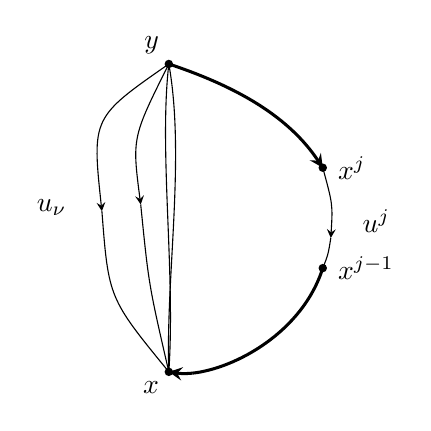
\begin{tikzpicture}[>=stealth,scale=0.85]
  \fill (0,2.3) circle (1.8pt);%
  \fill (0,-2.3) circle (1.8pt);%
  \fill (2.3,0.75) circle (1.8pt);%
  \fill (2.3,-0.75) circle (1.8pt);%
  \node[above left] at (0,2.3) {$y$};
  \node[below left] at (0,-2.3) {$x$};
  \node[right=2pt] at (2.3,0.75) {$x^{j}$};
  \node[right=2pt] at (2.3,-0.75) {$x^{j-1}$};
  \draw[->] (0,2.3) .. controls (-1.15,1.5) .. (-1.0,0.1);%
  \draw (-1.0,0.1) .. controls (-0.9,-1.2) .. (0,-2.3);%
  \node at (-1.75,0.15) {$u_{\nu}$};
  \draw[->] (0,2.3) .. controls (-0.55,1.2) .. (-0.42,0.2);%
  \draw (-0.42,0.2) .. controls (-0.3,-1.0) .. (0,-2.3);%
  \draw (0,2.3) .. controls (-0.15,1.0) and (0.1,-0.8) .. (0,-2.3);%
  \draw (0,2.3) .. controls (0.25,0.9) and (-0.05,-0.9) .. (0,-2.3);%
  \draw[line width=1.1pt,->] (0,2.3) .. controls (1.05,1.95) and (1.8,1.5) .. (2.3,0.75);%
  \draw[->] (2.3,0.75) .. controls (2.45,0.2) .. (2.42,-0.3);%
  \draw (2.42,-0.3) .. controls (2.38,-0.55) .. (2.3,-0.75);%
  \node at (3.1,-0.05) {$u^{j}$};
  \draw[line width=1.1pt] (2.3,-0.75) .. controls (2.0,-1.7) and (1.0,-2.25) .. (0.35,-2.32);%
  \draw[line width=1.1pt,->] (0.35,-2.32) .. controls (0.2,-2.33) .. (0,-2.3);%
\end{tikzpicture}

图 6.10
\end{minipage}

在合适的泛函分析框架中使用\trFredholm{}理论，可以证明：对 $(H,J)$ 的一个%
通有选取，诸集合 $\mathcal{M}(y,x)$ 是\trSmooth{}的有限维\trManifold。把方程%
\eqref{eq:floer-pde} 沿 $u$ 的\trVectorField{} $\xi\in C^{\infty}(u^{*}TM)$%
方向\trLinearization，便导出线性一阶微分\trOperator
\begin{equation}\label{eq:floer-linearized-F}
F(u)\xi\ :=\ \nabla_{s}\xi\ +\ J(u)\nabla_{t}\xi\ +\ \nabla_{\xi}J(u)\,\frac{\partial u}{\partial t}\ +\ \nabla_{\xi}\nabla H(t,u)\,,
\end{equation}
其中 $\nabla_{s}$、$\nabla_{t}$、$\nabla_{\xi}$ 表示关于由 $J$ 相配的度量 $g$%
的协变导数。若 $u:\R\times S^{1}\to M$ 是连接 $y$ 与 $x$ 的任一\trSmooth{}%
映射（从而对两个\trNondegenerate{}解 $y,x\in\mathcal{P}_{H}$ 满足%
\eqref{eq:floer-asymptotic}），则 $F(u)$ 是适当的\trSobolev{}空间之间的一个%
\trFredholm{}算子。带有满足 \eqref{eq:floer-metric-g} 的%
\trAlmostComplexStructure{} $J$ 的对 $(H,J)$ 称为正则的，如果 $F(u)$ 对每个%
$u\in\mathcal{M}$ 都是满射的线性算子。利用\trSard-\trSmale{}定理可以证明，正则对之集关于 $C^{\infty}$-\trTopology{}%
是\trDense{}的。于是由%
\trImplicitFunctionTheorem{}得出：$\mathcal{M}(y,x)$ 的确是一个\trSmooth{}%
\trManifold，其在 $u\in\mathcal{M}(y,x)$ 附近的局部维数为
\begin{equation}\label{eq:floer-dim-myx}
\dim\mathcal{M}(y,x)\ =\ \operatorname{Index}F(u)\,.
\end{equation}
如果我们除 \eqref{eq:floer-omega-spheres} 之外还要求 $(TM,J)$ 的第一%
\trChern{}类在 $\pi_{2}(M)$ 上为零，那么这个指数只依赖于 $u$ 的边界条件，即%
只依赖于 $y,x\in\mathcal{P}_{H}$。注意，$\omega$ 在同伦的意义下唯一地确定一%
个满足 \eqref{eq:floer-metric-g} 的\trAlmostComplexStructure{} $J$，我们以%
$c_{1}=c_{1}(TM)\in H^{2}(M)$ 表示 $TM$ 的第一\trChern{}类。我们将假设%
$[c_{1}]\big|_{\pi_{2}(M)}=0$，这要求代表 $c_{1}$ 的闭 2-形式在每张%
球面上的\trIntegral{}为零\footnote{原书印作「2-形式 $c_{1}$」，而 $c_{1}\in H^{2}(M)$%
 系上同调类而非具体的微分形式，当为「代表 $c_{1}$ 的闭 2-形式」，此处径改。%
——译者注}
\begin{equation}\label{eq:floer-c1-spheres}
\int_{S^{2}}u^{*}c_{1}\ =\ 0\,,\qquad u:S^{2}\to M\,.
\end{equation}

考虑一条\trNondegenerate\trPeriodicOrbit{} $x\in\mathcal{P}_{H}$。由于%
$x:S^{1}\to M$ 可缩，我们可以把它延拓成闭\trDisc{} $D$ 的一个映射%
$u:D\to M$，满足 $u\big|_{\partial D}=x$。现在取 $u^{*}(TM)$ 的一个%
\textbf{\trTrivialization}（trivialization）；它确定了 $x^{*}(TM)$ 的一个\trTrivialization。注意，%
若取 $x$ 的另一个延拓 $v:D\to M$，我们便得到 $x^{*}(TM)$ 的另一个\trTrivialization，%
然而由假设 $[c_{1}]\big|_{\pi_{2}(M)}=0$，它与前者\trHomotopic。在\trTrivialization{}了%
的切丛 $x^{*}(TM)$ 中，\trHamiltonianVectorField{} $X_{H}$ 沿 $x$ 的%
\trLinearization\trFlow{}确定了一个伴随 $x$ 的唯一\trMaslov{}型指数%
$\mu(H,x)\in\Z$。（诸整数与 $(\R^{2n},\omega_{0})$ 上关于时间\trPeriodic{}且%
\trNondegenerate{}的线性\trHamiltonianSystem{}的\trHomotopy{}类一一对应。）%
这给出
\begin{equation}\label{eq:floer-muH-map}
\mu_{H}\ :\ \mathcal{P}_{H}\ \longrightarrow\ \Z\,,\qquad x\ \mapsto\ \mu(H,x)\,.
\end{equation}
若\trSmooth{}映射 $u:\R\times S^{1}\to M$ 对\trHamiltonianVectorField{}的两个%
\trNondegenerate\trPeriodicSolution{} $y,x\in\mathcal{P}_{H}$ 满足%
\eqref{eq:floer-asymptotic}，则 $F(u)$ 的\trFredholm{}指数由下式给出
\begin{equation}\label{eq:floer-index-formula}
\operatorname{Index}F(u)\ =\ \mu(H,y)-\mu(H,x)\,.
\end{equation}
于是对通有的对 $(H,J)$ 我们得出 $\dim\mathcal{M}(y,x)=\mu_{H}(y)-\mu_{H}(x)$。%
关于指数 $\mu_{H}$ 的定义以及上述指数公式的一个证明，我们参考%
D.~\trSalamon{}与 E.~\trZehnder{} [190]。我们指出，若%
$[c_{1}]\big|_{\pi_{2}(M)}\neq0$，指数 \eqref{eq:floer-muH-map} 将依赖于所选%
延拓的\trHomotopy{}类。这种不确定性将是整数 $2N$，此处%
$N\Z=\bigl\{(u^{*}c_{1})[S^{2}]\ \bigm|\ u\in\pi_{2}(M)\bigr\}$。因此%
$\mu(H)$ 只能作为映射 $\mu_{H}:\mathcal{P}_{H}\to\Z/2N\Z$ 而良定。

我们现在已准备好定义联系于 $(M,\omega)$ 上正则对 $(H,J)$ 的\trFloer{}同调群。%
以 $C=C(M,H)$ 表示由\trHamiltonianVectorField{}的非退化可缩%
\trPeriodicOrbit{}之集 $\mathcal{P}_{H}$ 中那有限多个元素在 $\Z_{2}$ 上生成的%
向量空间。这个向量空间带有由指数映射 $\mu:\mathcal{P}_{H}\to\Z$ 定义的分次：
\begin{equation}\label{eq:floer-chain-C}
\begin{aligned}
C\ &=\ \bigoplus_{k\in\Z}C_{k}\\
C_{k}\ &=\ C_{k}(M,H)\ =\ \operatorname{span}_{\Z_{2}}\bigl\{x\in\mathcal{P}_{H}\ \bigm|\ \mu(x,H)=k\bigr\}\,.
\end{aligned}
\end{equation}
现在考虑满足 $\mu(y)-\mu(x)=1$ 的 $y,x\in\mathcal{P}_{H}$。那么\trManifold{}%
$\mathcal{M}(y,x)$ 是一维的，即 $\dim\mathcal{M}(y,x)=1$。鉴于\trCompactness{}%
并结合流形结构，可以证明 [85]：这个\trManifold{}只有有限多个连通分支，每个%
分支由一条\trConnectingOrbit{}连同它在时间 $-s$ 平移下的全部像组成。\trFloer{}%
利用这一点构造了一个线性\textbf{\trBoundaryOperator}（boundary operator）%
$\partial:C\to C$，它通过以模 $2$ 计数\trConnectingOrbit{}来保持分次。映射%
$\partial_{k}=\partial_{k}(M,H,J):C_{k}\to C_{k-1}$ 定义为
\begin{equation}\label{eq:floer-boundary-op}
\partial_{k}y\ =\ \sum_{\{x\in\mathcal{P}_{H}\,|\,\mu(x)=k-1\}}\langle\partial y,x\rangle\,x\,,
\end{equation}
其中 $y\in\mathcal{P}_{H}$ 满足 $\mu(y)=k$。矩阵元素%
$\langle\partial y,x\rangle\in\Z_{2}$ 是 $\mathcal{M}(y,x)$ 的连通分支按模%
$2$ 计数的数目。\trFloer{}证明了 [85]：$\partial\circ\partial=0$，从而对%
$(C,\partial)$ 定义了一个链复形。它的同调
\begin{equation}\label{eq:floer-homology-HF}
HF_{k}(M,H,J)\ :=\ \frac{\ker\bigl(\partial:C_{k}\to C_{k-1}\bigr)}{\operatorname{im}\bigl(\partial:C_{k+1}\to C_{k}\bigr)}
\end{equation}
称为 $(M,\omega)$ 上对 $(H,J)$ 的\trFloer{}同调。

为了解释边缘算子 $\partial_{k+1}:C_{k+1}\to C_{k}$ 的关系%
$\partial_{k}\circ\partial_{k+1}=0$，我们取 $x\in C_{k+1}$、$y\in C_{k}$ 与%
$z\in C_{k-1}$。设存在连接 $u\in\mathcal{M}(x,y)$ 与 $v\in\mathcal{M}(y,z)$。%
那么我们可以把对 $(u,v)$ 看成连接 $x$ 与 $z$ 的一条\textbf{「\trBrokenTrajectory」}%
（broken trajectory）。借一种称为\textbf{\trGluingMethod}（gluing method）的%
\trPerturbation{}论证，\trFloer{}在 [85] 中建立了 $\mathcal{M}(x,z)$ 中一个%
唯一的、由相伴真连接组成的一参数族。对时间 $s$ 平移的 $\R$-作用取商，我们就%
这样得到一个无\trBoundary{}的、由未参数化\trOrbit{}组成的连通一维\trManifold，%
它表示 $\mathcal{M}(x,z)$ 的一个连通分支。这样的一维\trManifold{}或是圆周，%
或是与开区间同胚、具有两个端（end）的流形。%
\cref{prop:broken-orbit-compactness}中的%
\trCompactness{}论证表明：每个端都在适当的意义下收敛到一条良定的破裂%
\trTrajectory{} $(u',v')\in\mathcal{M}(x,y')\times\mathcal{M}(y',z)$，对某个%
$y'\in C_{k}$。粘合构造又在相反的过程中表明，诸破裂\trTrajectory{}与这样的%
端一一对应。于是，一维\trManifold{} $\mathcal{M}(x,z)/\R$ 有偶数个端。

\begin{center}
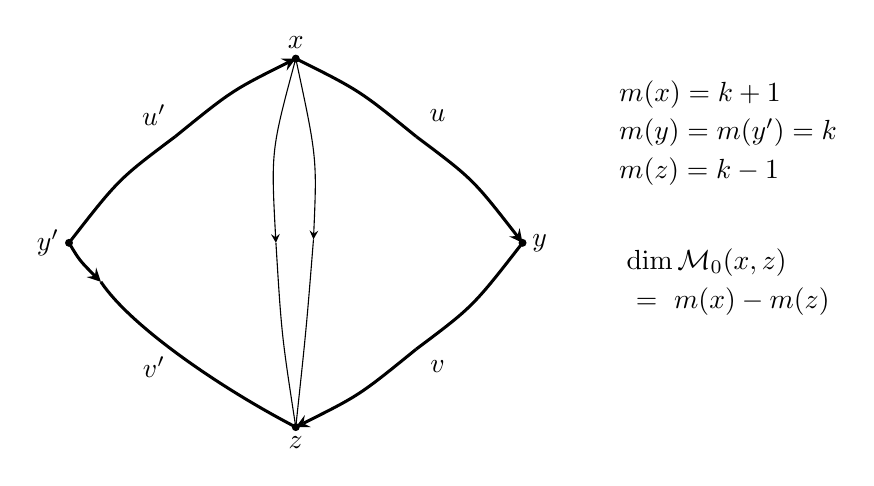
\begin{tikzpicture}[>=stealth,scale=0.9]
  \fill (0,2.6) circle (1.6pt);%
  \node[above] at (0,2.6) {$x$};
  \fill (0,-2.6) circle (1.6pt);%
  \node[below] at (0,-2.6) {$z$};
  \fill (3.2,0) circle (1.6pt);%
  \node[right] at (3.2,0) {$y$};
  \fill (-3.2,0) circle (1.6pt);%
  \node[left] at (-3.2,0) {$y'$};
  \draw[line width=1.1pt] (0,2.6) .. controls (0.9,2.15) .. (1.7,1.5);%
  \draw[line width=1.1pt,->] (1.7,1.5) .. controls (2.5,0.9) .. (3.2,0);%
  \node at (2.0,1.8) {$u$};
  \draw[line width=1.1pt] (-3.2,0) .. controls (-2.5,0.9) .. (-1.7,1.5);%
  \draw[line width=1.1pt,->] (-1.7,1.5) .. controls (-0.9,2.15) .. (0,2.6);%
  \node at (-2.0,1.8) {$u'$};
  \draw[line width=1.1pt] (3.2,0) .. controls (2.5,-0.9) .. (1.7,-1.5);%
  \draw[line width=1.1pt,->] (1.7,-1.5) .. controls (0.9,-2.15) .. (0,-2.6);%
  \node at (2.0,-1.75) {$v$};
  \draw[line width=1.1pt,->] (-3.2,0) .. controls (-3.05,-0.25) .. (-2.75,-0.55);%
  \draw[line width=1.1pt] (-2.75,-0.55) .. controls (-2.35,-1.15) and (-1.15,-2.0) .. (0,-2.6);%
  \node at (-2.0,-1.75) {$v'$};
  \draw[->] (0,2.6) .. controls (-0.35,1.3) .. (-0.28,0.0);%
  \draw (-0.28,0.0) .. controls (-0.2,-1.3) .. (0,-2.6);
  \draw[->] (0,2.6) .. controls (0.3,1.2) .. (0.25,0.05);%
  \draw (0.25,0.05) .. controls (0.15,-1.2) .. (0,-2.6);
  \node[align=left] at (6.1,1.55) {$m(x)=k+1$\\[2pt] $m(y)=m(y')=k$\\[2pt] $m(z)=k-1$};
  \node[align=left] at (6.1,-0.55) {$\dim\mathcal{M}_{0}(x,z)$\\[2pt] $\ =\ m(x)-m(z)$};
\end{tikzpicture}
\end{center}

因此，介于 $x$ 与 $z$ 之间的诸「破裂\trTrajectory」$(u,v)$ 成对出现。由于%
我们使用 $\Z_{2}$ 系数，对每个 $x\in C_{k+1}$ 我们得到
\[
\sum_{m(z)=k-1}\ \Biggl(\ \sum_{m(y)=k}\ \langle\partial x,y\rangle\langle\partial y,z\rangle\ \Biggr)\,z\ =\ 0\,.
\]
关于这一粘合构造的繁难细节，我们参考 A.~\trFloer{} [85] 与 C.~\trTaubes{}%
[210, 211]，特别是 M.~\trSchwarz{}的新近专著 [191]。

链复形由有界\trOrbit{}的解空间 $\mathcal{M}$ 的一维连通分支定义。它的构造%
显然类似于有限维\trCompact\trManifold{}上\trMorse-\trSmale\trGradient\trFlow{}%
的那个熟悉的\trMorse{}复形。\trMorse-\trSmale{}流的横截性条件对应于%
「\trFredholm{}算子 $F(u)$ 是满射映射」这一假设，后者如有限维情形一样只在%
「通有」意义下成立。\trMorse-\trSmale{}流的\trNondegenerate\trCriticalPoint{}%
的\trMorseIndex{}这一角色，由伴随\trNondegenerate{}可缩\trPeriodicOrbit{}%
$x\in\mathcal{P}_{H}$ 的整数 $\mu(x,H)$ 扮演。而 $x\in\mathcal{P}_{H}$ 的%
\trMorseIndex{}是无穷大！

到目前为止，$\mathcal{M}$ 有可能是空的、诸\trFloer{}同调群有可能是平凡的。%
此时回忆 C.~\trConley{}关于\trCompact{}空间上\trFlow{}的\trConley{}指数%
理论的一个至关重要的方面是有益的：该理论的设计方式使它在\trContinuation{}下%
\trInvariant。受这一理论的启发，\trFloer{}为他的同调群建立了一条类似的同伦%
不变性，利用它可以证明这些群与构造时所用的 $(H,J)$ 无关。$H$ 与 $J$ 的一个%
特殊选取随即使得他得以计算该同调：

\begin{theorem}[\trFloer\trContinuation]\label{thm:floer-continuation}
对每两个正则对 $(H^{\alpha},J^{\alpha})$ 与 $(H^{\beta},J^{\beta})$，存在%
\trFloer{}同调的一个自然同构，它保持分次
\[
\psi^{\beta\alpha}\ :\ HF_{*}\bigl(M,H^{\alpha},J^{\alpha}\bigr)\ \longrightarrow\ HF_{*}\bigl(M,H^{\beta},J^{\beta}\bigr)\,.
\]
此外，若 $(H^{\gamma},J^{\gamma})$ 是另一个正则对，则
\[
\psi^{\alpha\beta}\circ\psi^{\beta\gamma}\ =\ \psi^{\alpha\gamma}\qquad\text{而}\qquad \psi^{\alpha\alpha}\ =\ \id\,.
\]
\end{theorem}

我们看到，\trFloer{}同调 $HF_{*}(M,H,J)$ 与构造 $\mathcal{P}_{H}$ 之%
\trConnectingOrbit{}时所用的正则对 $(H,J)$ 无关；因此它是底\trManifold{}%
$(M,\omega)$ 的一个\trInvariant{}量。我们有一个范畴，其对象是与正则对%
$(H,J)$ 相伴的诸\trFloer{}同调群，其态射是由正则同伦（下文将作解释）诱导的%
自然同构 $\psi^{\beta\alpha}$。用 C.~\trConley{} [54] 的术语，这样一个任意%
两个对象之间恰有一个态射的范畴称为一个\textbf{\trConnectedSimpleSystem}%
（connected simple system）。

我们将勾画其证明的思想，它同样基于一个偏微分方程的特殊解与\trFredholm{}%
理论。我们循 D.~\trSalamon{}与 E.~\trZehnder{} [190] 的表述。为了构造同态%
$\varphi^{\beta\alpha}:C(M,H^{\alpha},J^{\alpha})\to C(M,H^{\beta},J^{\beta})$，%
我们选取一个由\trHamiltonian{}函数组成的\trSmooth{}同伦%
$H^{\alpha\beta}:\R\times S^{1}\times M\to\R$，连同\trAlmostComplexStructure{}%
的一个\trSmooth{}同伦 $J^{\alpha\beta}:\R\times M\to\operatorname{End}(TM)$，%
使得当 $|s|$ 充分大时 $H^{\alpha\beta}(s,t,x)$ 与 $J^{\alpha\beta}(s,x)$ 不%
依赖于 $s$，且满足
\begin{equation}\label{eq:floer-homotopy-H}
\begin{aligned}
\lim_{s\to-\infty}H^{\alpha\beta}(s,t,x)\ &=\ H^{\alpha}(t,x)\\
\lim_{s\to+\infty}H^{\alpha\beta}(s,t,x)\ &=\ H^{\beta}(t,x)
\end{aligned}
\end{equation}
以及\footnote{原书 \eqref{eq:floer-homotopy-J} 第二行印作%
「$J^{\alpha\beta}(s,t,x)$」，依上文定义（$J^{\alpha\beta}:\R\times M\to%
\operatorname{End}(TM)$）疑为「$(s,x)$」之误，此处径改。——译者注}
\begin{equation}\label{eq:floer-homotopy-J}
\begin{aligned}
\lim_{s\to-\infty}J^{\alpha\beta}(s,x)\ &=\ J^{\alpha}(x)\\
\lim_{s\to+\infty}J^{\alpha\beta}(s,x)\ &=\ J^{\beta}(x)\,.
\end{aligned}
\end{equation}
回忆：与 $\omega$ \trCompatible{}的\trAlmostComplexStructure{}之空间是可缩的。%
给定这样一对连接资料的同伦 $(H^{\alpha\beta},J^{\alpha\beta})$，我们研究偏%
微分方程
\begin{equation}\label{eq:floer-homotopy-pde}
\frac{\partial u}{\partial s}\ +\ J(s,u)\frac{\partial u}{\partial t}\ +\ \nabla H(s,t,u)\ =\ 0
\end{equation}
的\trSmooth{}解 $u(s,t)$，$u:\R\times S^{1}\to M$，它们满足渐近边界条件
\begin{equation}\label{eq:floer-homotopy-bc}
\lim_{s\to-\infty}u(s,t)\ =\ x^{\alpha}(t)\,,\qquad \lim_{s\to+\infty}u(s,t)\ =\ x^{\beta}(t)
\end{equation}
其中 $x^{\alpha}\in\mathcal{P}_{H^{\alpha}}$，$x^{\beta}\in\mathcal{P}_{H^{\beta}}$。

这些解可以视为一个\trTimeDependent\trGradient\trFlow{}的\trFlow{}线，该%
\trFlow{}由\trActionFunctional{} $\varphi_{H_{s}}$ 定义，%
$H_{s}(t,x)=H^{\alpha\beta}(s,t,x)$，所用度量是由\trAlmostComplexStructure{}%
$J_{s}$ 确定的\trTimeDependent{}度量。与前面一样，有界能量的解满足边界条件。%
我们将缩记
\begin{equation}\label{eq:floer-M-alpha-beta}
\mathcal{M}\bigl(x^{\alpha},x^{\beta},H^{\alpha\beta},J^{\alpha\beta}\bigr)
\end{equation}
为 \eqref{eq:floer-homotopy-pde} 与 \eqref{eq:floer-homotopy-bc} 的\trSmooth{}%
解 $u:\R\times S^{1}\to M$ 之集。这个集通过把方程沿 $u$ 的\trVectorField{}%
$\xi\in C^{\infty}(u^{*}TM)$ 方向\trLinearization{}而得到局部分析，这导出%
适当\trSobolev{}空间之间的一个线性算子%
$F^{\beta\alpha}(u):W^{k,p}(u^{*}TM)\to W^{k-1,p}(u^{*}TM)$。对每个满足边界%
条件 \eqref{eq:floer-homotopy-bc}（其中 $x^{\alpha},x^{\beta}$%
\trNondegenerate）的\trSmooth{}映射 $u:\R\times S^{1}\to M$，算子%
$F^{\beta\alpha}(u)$ 是\trFredholm{}的，其指数算得为
\begin{equation}\label{eq:floer-index-fba}
\operatorname{Index}F^{\beta\alpha}(u)\ =\ \mu\bigl(x^{\alpha},H^{\alpha}\bigr)-\mu\bigl(x^{\beta},H^{\beta}\bigr)\,.
\end{equation}
此外，对从 $(H^{\alpha},J^{\alpha})$ 到 $(H^{\beta},J^{\beta})$ 的一个正则%
同伦，该算子是满射的。这里，一对 $(H^{\alpha\beta},J^{\alpha\beta})$ 称为%
正则的，如果两对 $(H^{\alpha},J^{\alpha})$ 与 $(H^{\beta},J^{\beta})$ 都%
正则，且线性算子 $F^{\beta\alpha}(u)$ 对 \eqref{eq:floer-homotopy-pde} 与%
\eqref{eq:floer-homotopy-bc} 的每个解 $u$（其中 $x^{\alpha}\in\mathcal{P}_{H^{\alpha}}$%
与 $x^{\beta}\in\mathcal{P}_{H^{\beta}}$ 任取）都是满射的。\trFloer{}证明了%
[84, 85]：连接正则对的正则同伦之集，在全体连接 $(H^{\alpha},J^{\alpha})$ 到%
$(H^{\beta},J^{\beta})$\footnote{原书印作「connecting $(H^{\alpha},J^{\alpha})$%
 to $(H^{\beta},J^{\alpha})$」，末对依上下文疑为「$(H^{\beta},J^{\beta})$」之%
误，此处径改。——译者注} 的\trSmooth{}同伦之集中关于 $C^{\infty}$-\trTopology{}%
是\trDense{}的。（\trFloer{}是对\trLagrange{}交的类似几何问题实施其证明的。）%
于是得出：\trConnectingOrbit{}的空间%
$\mathcal{M}(x^{\alpha},x^{\beta},H^{\alpha\beta},J^{\alpha\beta})$ 是一个%
有限维\trManifold{}，且
\begin{equation}\label{eq:floer-dim-mab}
\dim\mathcal{M}\bigl(x^{\alpha},x^{\beta},H^{\alpha\beta},J^{\alpha\beta}\bigr)\ =\ \mu\bigl(x^{\alpha},H^{\alpha}\bigr)-\mu\bigl(x^{\beta},H^{\beta}\bigr)\,.
\end{equation}
这使我们得以构造一个\trChainMap
\[
\varphi^{\beta\alpha}=\varphi\bigl(H^{\alpha\beta},J^{\alpha\beta}\bigr):C_{k}\bigl(M,H^{\alpha}\bigr)\longrightarrow C_{k}\bigl(M,H^{\beta}\bigr)
\]
它以模 $2$ 计数具有相同指数的\trPeriodicSolution{}之间的\trConnectingOrbit：
\begin{equation}\label{eq:floer-chain-map}
\varphi^{\beta\alpha}\bigl(x^{\alpha}\bigr)\ =\ \sum_{\mu(x^{\beta},H^{\beta})=k}\Bigl\langle\varphi^{\beta\alpha}\bigl(x^{\alpha}\bigr),x^{\beta}\Bigr\rangle x^{\beta}\,,
\end{equation}
其中 $\mu(x^{\alpha},H^{\alpha})=k$，而%
$\bigl\langle\varphi^{\beta\alpha}(x^{\alpha}),x^{\beta}\bigr\rangle$\footnote{%
原书印作「$\langle\varphi^{\beta\alpha}x^{\alpha},x^{\beta}\rangle$」，缺括号，%
依 \eqref{eq:floer-chain-map} 式内补全，此处径改。——译者注} 是按模%
$2$ 计的解数。

可以证明：对每个正则同伦，这个线性映射 $\varphi^{\beta\alpha}$ 都是\trChainMap，即满足 $\partial^{\beta}\varphi^{\beta\alpha}=\varphi^{\beta\alpha}\partial^{\alpha}$；%
此外它保持分次。因此它诱导了\trFloer{}同调的一个自然同态 $\psi^{\beta\alpha}$，%
而且结果表明它与同伦 $(H^{\alpha\beta},J^{\alpha\beta})$ 的选取无关。说得更%
精确些，可以证明：对从 $(H^{\alpha},J^{\alpha})$ 到 $(H^{\beta},J^{\beta})$%
的两个正则同伦 $(H_{0}^{\alpha\beta},J_{0}^{\alpha\beta})$ 与%
$(H_{1}^{\alpha\beta},J_{1}^{\alpha\beta})$，相伴的\trChainMap $\varphi_{0}^{\beta\alpha}$%
与 $\varphi_{1}^{\beta\alpha}$ 是链同伦（chain homotopic）的\footnote{原书印作%
「chain homotopy equivalent（链同伦等价）」，系非标准措辞：两个链映射之间的%
关系应为「链同伦」，「链同伦等价」通常指两个链复形之间存在互为链同伦逆的%
链映射，此处径改。——译者注}。这便结束了我们对%
\cref{thm:floer-continuation}的勾画。

最后，为了计算同调，\trFloer{}使用了\trContinuation{}定理，把一个正则对%
$(H^{\alpha},J^{\alpha})$ 与一个非常特殊的对 $(H,J)$ 连接起来，后者的%
\trFloer{}同调等同于由函数 $H:M\to\R$ 的\trGradient\trFlow{}在底\trManifold{}%
$M$ 上定义的\trMorse{}复形的同调。

\noindent\begin{minipage}{\linewidth}
\centering
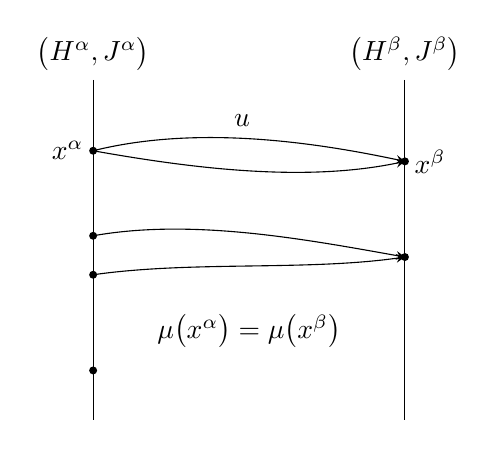
\begin{tikzpicture}[>=stealth,scale=0.9]
  \draw (0,2.2) -- (0,-2.6);%
  \draw (4.4,2.2) -- (4.4,-2.6);%
  \node[above] at (0,2.2) {$\bigl(H^{\alpha},J^{\alpha}\bigr)$};
  \node[above] at (4.4,2.2) {$\bigl(H^{\beta},J^{\beta}\bigr)$};
  \fill (0,1.2) circle (1.6pt);%
  \node[left] at (0,1.2) {$x^{\alpha}$};
  \fill (4.4,1.05) circle (1.6pt);%
  \node[right] at (4.4,1.05) {$x^{\beta}$};
  \fill (0,0.0) circle (1.6pt);%
  \fill (0,-0.55) circle (1.6pt);%
  \fill (0,-1.9) circle (1.6pt);%
  \fill (4.4,-0.3) circle (1.6pt);%
  \draw[->] (0,1.2) .. controls (1.4,1.55) and (3.0,1.35) .. (4.4,1.05);%
  \draw[->] (0,1.2) .. controls (1.4,0.95) and (3.0,0.75) .. (4.4,1.05);%
  \node at (2.1,1.62) {$u$};
  \draw[->] (0,0.0) .. controls (1.4,0.25) and (3.0,-0.05) .. (4.4,-0.3);%
  \draw[->] (0,-0.55) .. controls (1.4,-0.35) and (3.0,-0.5) .. (4.4,-0.3);%
  \node at (2.2,-1.35) {$\mu\bigl(x^{\alpha}\bigr)=\mu\bigl(x^{\beta}\bigr)$};
\end{tikzpicture}

图 6.11
\end{minipage}

\begin{theorem}[同调的计算]\label{thm:floer-homology-computation}
对每个正则对 $(H^{\alpha},J^{\alpha})$，存在一个自然同构
\[
\psi^{\alpha}\ :\ HF_{*}\bigl(M,H^{\alpha},J^{\alpha}\bigr)\ \longrightarrow\ H_{*}\bigl(M,\Z_{2}\bigr),
\]
它保持分次%
\[
\psi^{\alpha}_{k}\ :\ HF_{k}\bigl(M,H^{\alpha},J^{\alpha}\bigr)\ \longrightarrow\ H_{k+n}\bigl(M,\Z_{2}\bigr)
\]
——此同构联系着对 $(H^{\alpha},J^{\alpha})$ 的\trFloer{}同调与 $M$ 的带%
$\Z_{2}$ 系数的\trSingularHomology。此外，若 $(H^{\beta},J^{\beta})$ 是另一%
个正则对，则
\[
\psi^{\alpha}\ =\ \psi^{\beta}\circ\psi^{\beta\alpha}\,.
\]
特别地，\trFloer{}同调在 $|k|>n$ 时为零。
\end{theorem}

我们概述 \cref{thm:floer-homology-computation} 的证明思想，循 [190] 的表述。%
我们选取一个特殊的\trHamiltonian{}函数 $H:M\to\R$，它不依赖于时间 $t$，并且%
是一个\trMorse{}函数，使得其在 $M$ 上的全部\trCriticalPoint{}都%
\trNondegenerate。此外，我们假设 $H$ 在 $C^{2}$ \trTopology{}下充分小。于是，%
正如我们在上文所见，$M$ 上\trHamiltonianSystem{} $\dot{x}=X_{H}(x)$ 的周期为%
$1$ 的\trPeriodicSolution{}都是常值的，并与 $H$ 的\trCriticalPoint{}一致，%
从而在这种情形
\begin{equation}\label{eq:floer-PH-small}
\mathcal{P}_{H}\ =\ \bigl\{\,x(t)=x\in M\ \bigm|\ dH(x)=0\,\bigr\}\,.
\end{equation}
在「小」\trHamiltonian{} $H$ 的这一局面下，$H$ 的\trCriticalPoint{} $x$ 的%
\trMorseIndex{} $\operatorname{ind}_{H}(x)$ 与 $\dot{x}=X_{H}(x)$ 的常值%
$1$-\trPeriodicSolution{} $x(t)=x$ 的指数 $\mu(x,H)$ 之间的关系为
\begin{equation}\label{eq:floer-index-shift}
\mu(x,H)\ =\ \operatorname{ind}_{H}(x)-n\,,\qquad x\in\mathcal{P}_{H}\,,
\end{equation}
见 [190]。我们可以选取一个\trAlmostComplexStructure{} $J$，使得 $(H,J)$ 是%
一个正则对。于是可以证明：对满足 $\mu(y,H)-\mu(x,H)=1$ 的%
$x,y\in\mathcal{P}_{H}$，偏微分方程 \eqref{eq:floer-pde} 与%
\eqref{eq:floer-asymptotic} 的解 $u\in\mathcal{M}(y,x)$ 也与时间 $t$ 无关。%
于是令 $u(s,t)=\gamma(s)$，它们便满足\trGradient{}方程
\begin{equation}\label{eq:floer-grad-flow-gamma}
\frac{d\gamma}{ds}\ +\ \nabla H\Bigl(\gamma(s)\Bigr)\ =\ 0\quad\text{于 }M\,,
\end{equation}
以及边界条件：当 $s\to-\infty$ 时 $\gamma(s)\to y$，当 $s\to+\infty$ 时%
$\gamma(s)\to x$。只要 $\operatorname{ind}F(u)=\operatorname{ind}_{H}(y)-%
\operatorname{ind}_{H}(x)=1$，这些解正是\trMorse-\trSmale\trGradient\trFlow{}%
$\dot{x}=-\nabla H(x)$ 的一维\trConnectingOrbit，具体有
\begin{equation}\label{eq:floer-myx-ws}
\mathcal{M}(y,x)\ =\ W^{u}(y)\ \cap\ W^{s}(x)\,,
\end{equation}
于是，链复形 $C(M,H)$ 与那个熟悉的\trMorse{}复形一致，在后者中%
$C_{k}(H)=\operatorname{span}_{\Z_{2}}\bigl\{x\in M\ \bigm|\ dH(x)=0$ 且 $\operatorname{ind}_{H}(x)=k\bigr\}$\footnote{原书印作「$C_{k}(H)=\{x\in M\mid dH(x)=0$ 且 $\operatorname{ind}_{H}(x)=k\}$」，漏写张成记号：$C_{k}(H)$ 系链群（向量空间）而非点集，与本节 \eqref{eq:floer-chain-C} 之定义一致，此处补 $\operatorname{span}_{\Z_{2}}$ 径改。——译者注}，%
而如上定义的边缘算子 $\partial_{k}=\partial_{k}(H,J):C_{k}\to C_{k-1}$ 以%
（模 $2$）计数 $M$ 上\trGradient\trFlow{}的\trConnectingOrbit。众所周知，它%
的同调群
\begin{equation}\label{eq:floer-morse-homology}
HM_{k}(M,H,J)\ =\ \frac{\ker\partial_{k}}{\operatorname{im}\partial_{k+1}}
\end{equation}
与 $M$ 的\trSingularHomology{}一致：
\begin{equation}\label{eq:floer-morse-singular}
HM_{k}(M,H,J)\ \cong\ H_{k}\bigl(M,\Z_{2}\bigr)\,.
\end{equation}
关于证明，我们参考 D.~\trSalamon{} [188] 以及 M.~\trSchwarz{}的新近专著%
[191]，后者在有限维\trManifold{}上基于\trMorse{}函数的\trTrajectory{}空间%
发展了一种\trMorse{}同调理论。鉴于 \eqref{eq:floer-index-shift} 我们看到，%
\trFloer{}为我们的特殊\trSymplecticManifold{} $(M,\omega)$ 所建立的链复形，%
与函数之\trGradient\trFlow{}的那个熟悉的\trMorse{}复形一致，分次平移了 $n$：
\begin{equation}\label{eq:floer-grading-shift}
HF_{k}(M,H,J)\ \cong\ HM_{k+n}(M,H,J)\ \cong\ H_{n+k}\bigl(M,\Z_{2}\bigr)\,.
\end{equation}
因此，\trFloer{}的诸\trNondegenerate\trPeriodicSolution{}之间的%
\trConnectingOrbit{}可以充当底\trManifold{}的同调的一个模型。我们特别得出：
\begin{equation}\label{eq:floer-morse-equation}
\sum_{x\in\mathcal{P}_{H}}t^{\mu(x,H)}\ =\ P(t,M)\,t^{-n}\ +\ (1+t)Q(t)\,.
\end{equation}
这条\trMorse{}方程把具有指数 $\mu(x,H)\in\Z$ 的\trNondegenerate{}可缩%
\trPeriodicSolution{} $x\in\mathcal{P}_{H}$ 与由\trPoincare{}多项式%
$P(t,M)$ 所描述的 $M$ 的\trTopology{}联系起来。回忆我们对 $(M,\omega)$ 所作%
的假设 $\omega\big|_{\pi_{2}}=0=c_{1}\big|_{\pi_{2}}$。在时间无关且小的%
\trMorse{}函数 $H$ 的情形，方程 \eqref{eq:floer-morse-equation} 变成熟悉的%
\trMorse{}方程
\begin{equation}\label{eq:floer-morse-equation-classical}
\sum_{\nabla H(x)=0}t^{m(x)}\ =\ P(t,M)\ +\ (1+t)Q(t)
\end{equation}
它把函数 $H$ 的\trCriticalPoint{}与\trPoincare{}多项式 $P(t,M)$ 联系起来。%
特别地，我们从 \eqref{eq:floer-morse-equation} 得出

\begin{theorem}[\trFloer]\label{thm:floer-betti-lower-bound}
假设\trCompact\trSymplecticManifold{} $(M,\omega)$ 满足%
$\omega\big|_{\pi_{2}(M)}=0$ 与 $c_{1}\big|_{\pi_{2}(M)}=0$，再假设 $M$ 上的%
时间\trPeriodic\trHamiltonianVectorField{} $\dot{x}=X_{H}(x)$ 只拥有%
\trNondegenerate{}的 $1$-\trPeriodicSolution。那么其数目至少是 $M$ 的%
\trBettiNumber{}之和 $SB\bigl(M,\Z_{2}\bigr)$。
\end{theorem}

例如 $\pi_{2}\bigl(T^{2n}\bigr)=0$，故每个辛\trTorus{} $(T^{2n},\omega)$ 都%
满足\cref{thm:floer-betti-lower-bound}的假设。实际上，\trFloer{}在 [85] 中%
证明了一个更一般的结果，其中只假设 $(M,\omega)$ 是单调的，%
其意义为
\begin{equation}\label{eq:floer-monotone}
\int_{S^{2}}u^{*}c_{1}\ =\ \lambda\int_{S^{2}}u^{*}\omega\,,
\end{equation}
对每张球面 $u:S^{2}\to M$ 成立，其中 $\lambda>0$ 为常数。

更晚近，H.~\trHofer{}与 D.~\trSalamon{} [119] 成功地在假设
\begin{equation}\label{eq:floer-hofer-salamon}
\omega(A)\ \leq\ 0\quad\text{对每个满足 }3-n\leq c_{1}(A)<0\text{ 的 }A\in\pi_{2}(M)\,,
\end{equation}
之下定义了\trFloer{}同调群，并分别在 $c_{1}\big|_{\pi_{2}(M)}=0$ 的情形%
以及 $N\geq\frac{1}{2}\dim(M)$（其中 $N\Z=c_{1}\bigl(\pi_{2}(M)\bigr)\subset\Z$）%
的情形计算了它们，从而在这些情形证明了\trArnold{}猜想。他们证明，诸%
\trFloer{}群构成广义 Laurent 级数的\trNovikov{}环上的一个模。这样的环由%
S.~\trNovikov{}在其对闭\trOneForm{}的\trMorseTheory{}的推广中引入 [170]。在假设%
\eqref{eq:floer-hofer-salamon} 之下，所得到的理论是\trFloer{}同调的一个%
\trNovikov{}型变体。通过修改\trHofer{}与\trSalamon{}的思想，K.~\trOno{} [172]%
给出了\trFloer{}同调理论的一个修改构造，同样在假设%
\eqref{eq:floer-hofer-salamon} 之下，它可以无须附加假设而被计算。结果表明，%
对一个合适的系数域，这些\trFloer{}群同构于该\trManifold{}的\trSingularHomology%
群，从而特别地在维数 $2$、$4$ 与 $6$——\eqref{eq:floer-hofer-salamon} 在其中%
自动满足、不施加实质限制——建立了\trArnold{}猜想。满足条件 \eqref{eq:floer-hofer-salamon} 的%
\trManifold{}具有证明中用到的一个性质：对一个通有的\trAlmostComplexStructure，%
不存在负\trChern{}数的\trHolomorphic{}球面。

对一般的 $\dim M\geq8$ 的\trCompact\trSymplecticManifold，\trArnold{}猜想%
仍然开放。

应当指出，\trFloer{}同调群 $HF_{*}$ 可以对整系数 $\Z$（代替 $\Z_{2}$）从而%
对每个\trAbelian{}群定义。为此，必须对每条\trConnectingOrbit{} $u\in\mathcal{M}(y,x)$%
（只要 $\mu(y)-\mu(x)=1$）指定一个整数 $+1$ 或 $-1$。然而，这样一种定向的%
确定相当精妙，它要求\textbf{\trModuliSpace}（moduli space）$\mathcal{M}(y,x)$ 的一个%
相容定向，对此我们参考 A.~\trFloer{}与 H.~\trHofer{} [89]。于是，上述所有%
陈述不仅对 $\Z_{2}$ 系数成立，对 $\Z$ 系数也成立。

$M$ 上 $\dot{x}=X_{H}(x)$ 的诸 $1$-\trPeriodicSolution{}与\trHamiltonianMap{}%
$\psi^{1}$ 的诸\trFixedPoint{}一一对应，后者是%
\trHamiltonianVectorField{}所生成的\trFlow{}的\trTimeOneMap。由于 $M$%
\trCompact，鉴于\trPoincare{}\trRecurrence{}定理，除了这些\trFixedPoint{}之外，还应当%
预期存在大量具有大周期的\trPeriodic{}点。的确，若其中一个\trFixedPoint{}是%
引言中所解释的那种一般\trElliptic{}型的，则它是其他\trPeriodic{}点的聚点，后者的素%
周期趋于无穷。这由\trBirkhoff-\trLewis{}定理径直得出，这是一个局部定理，%
关于其证明我们参考 J.~\trMoser{} [164]。遗憾的是，我们对\trFixedPoint{}%
存在性的整体处理只给出关于其本性的很少信息，特别是没有给出为推演出附近%
\trPeriodic{}点所需的非线性\trBirkhoffInvariant{}的任何信息。接下来我们将%
在对诸 $1$-\trPeriodicSolution{}的附加假设下证明，从\trFloer{}同调可以推演%
出无穷多个\trPeriodicSolution。一个 $1$-\trPeriodicSolution{}%
$x(t)=x(t+1)$ 可以视为 $\tau$-\trPeriodicSolution{} $x(t)=x(t+\tau)$，%
对每个整数 $\tau\in\N$；此时它称为 $x$ 的 $\tau$ 次迭代解，记作 $x^{\tau}$。我们称%
一个 $1$-\trPeriodicSolution{} $x$ 为强\trNondegenerate{}的，如果它的全部%
迭代 $x^{\tau}$ 都\trNondegenerate，即如果
\[
\det\Bigl(1-d\psi^{\tau}\bigl(x(0)\bigr)\Bigr)\ \neq\ 0
\]
对一切正整数 $\tau$ 成立\footnote{原书此式印作「$\det\bigl(1-\psi^{\tau}(x(0))\bigr)\neq0$」，$\psi^{\tau}(x(0))$ 是一点而非线性映射，无从与恒同相减并取行列式，疑漏微分记号 $d$；依本节 \eqref{eq:floer-nondegen} 之式径改。——译者注}，而不仅对 $\tau=1$。

\begin{theorem}\label{thm:strongly-nondegenerate-infinite}
假设\trCompact\trSymplecticManifold{} $(M,\omega)$ 满足%
$\omega\big|_{\pi_{2}}=0$ 与 $c_{1}\big|_{\pi_{2}}=0$，并设%
$H:S^{1}\times M\to\R$ 是一个\trSmooth\trHamiltonian{}函数，使得%
\trHamiltonianSystem{}的全体可缩 $1$-\trPeriodicSolution{}都是强%
\trNondegenerate{}的。那么存在无穷多个具大整数周期的可缩%
\trPeriodicSolution。
\end{theorem}

这是 D.~\trSalamon{}与 E.~\trZehnder{}在 [190] 中证明的一个更一般陈述的%
特殊情形，后者只要求诸 $1$-\trPeriodicSolution{} $x(t)=x(t+1)$ 是弱%
\trNondegenerate{}的，即它们拥有至少一个不等于 $1$ 的\trFloquet{}乘子，使得%
$\sigma\bigl(d\psi^{1}(x(0))\bigr)\neq\{1\}$。$\pi_{2}(M)$ 上的条件无法去除，%
$M=S^{2}$ 上具无理频率的旋转一例（图 6.12）表明了这一点。

\noindent\begin{minipage}{\linewidth}
\centering
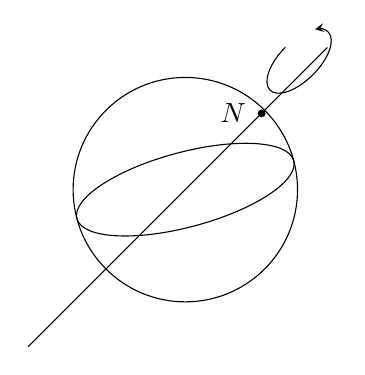
\begin{tikzpicture}[>=stealth,scale=0.95]
  \draw (-2.1,-2.1) -- (1.9,1.9);%
  \draw (0,0) circle (1.5);%
  \draw[rotate=15] (0,0) ellipse (1.5 and 0.5);%
  \fill (1.02,1.02) circle (1.5pt);%
  \node[left] at (0.94,1.02) {$N$};
  \begin{scope}[shift={(1.62,1.62)},rotate=45]%
    \draw[->] (0,0.4) arc (90:395:0.55 and 0.26);
  \end{scope}
\end{tikzpicture}

图 6.12
\end{minipage}

这是一个\trHamiltonianMap，却只有两个\trPeriodic{}点，即北极与南极处的强%
\trNondegenerate\trFixedPoint。

与这个例子形成鲜明对照的是，$S^{2}$ 的一个拥有 $\geq3$ 个\trFixedPoint{}的%
保面积\trDiffeomorphism{}自动拥有无穷多个\trPeriodic{}点。这一引人注目的%
现象由 J.M.~\trGambaudo{}与 P.~\trLeCalvez{} [103] 以及 J.~\trFranks{} [96]%
发现。人们不禁要猜想：\trCompact\trSymplecticManifold{} $(M,\omega)$ 上的%
每个\trHamiltonianMap，若其拥有的\trFixedPoint{}多于 V.~\trArnold{}猜想所%
必然要求的，就总拥有无穷多个\trPeriodic{}点。类似地，可以预期一张%
\trCompact{}且\trStrictlyConvex{}的\trHypersurface{} $S\subset\R^{4}$ 或%
携带 $2$ 条、或携带无穷多条\trClosedCharacteristic。

\cref{thm:strongly-nondegenerate-infinite}是\trFloer{}同调的一个简单推论。%
我们利用 [190] 中证明的一个事实：对强\trNondegenerate{}的%
$1$-\trPeriodicSolution{} $x(t)=x(t+1)$ 的指数 $\mu(x,H)$，下述迭代公式成立
\[
\mu\bigl(x^{\tau}\bigr)\ =\ \frac{1}{\pi}\Bigl(\tau\,\Delta(x)\ +\ r_{\tau}(x)\Bigr)\,.
\]
此处 $\Delta(x)\in\R$\footnote{原书文本层印作「$\vartheta(x)$」，页图实为%
「$\Delta(x)$」，此处从页图照录。——译者注} 是伴随该 $1$-\trPeriodicSolution{}%
的一个平均\trWindingNumber，而对每个 $\tau\in\N$ 有 $|r_{\tau}(x)|<\pi n$。%
我们看到，或者当 $\tau\to\infty$%
时 $|\mu(x^{\tau})|\to\infty$，或者对每个 $\tau$ 有 $|\mu(x^{\tau})|<n$。现在%
反设只有有限多个整数周期的\trPeriodicSolution。那么它们有一个公共周期，%
比如 $\tau_{0}\in\N$，我们取一个素数 $\tau>\tau_{0}$。于是%
$\dot{x}=X_{H}(x)$ 的全部 $\tau$-\trPeriodicSolution{}都是迭代的%
$1$-\trPeriodicSolution{}，从而由假设它们都\trNondegenerate。考虑%
$\mathcal{P}_{H}(\tau)$ 中诸 $\tau$-\trPeriodicSolution{}的\trFloer{}复形，%
我们得出
\[
\bigl|\mu(x)\bigr|\ \neq\ n\quad\text{对一切 }x\in\mathcal{P}_{H}(\tau)
\]
只要 $\tau$ 充分大。于是我们错过了最高与最低的同调群，这与\trMorse{}方程%
\eqref{eq:floer-morse-equation} 相矛盾。因此存在无穷多个%
\trPeriodicSolution。通过修改这一思想，[190] 中证明了：若只存在有限多个%
可缩 $1$-\trPeriodicSolution{} $x$——它们或许甚至\trDegenerate，但满足%
$\Delta(x)\neq0$——则对每个大且为素数的 $\tau\in\N$，存在一个可缩且以素数%
$\tau$ 为周期的 $\tau$-\trPeriodicSolution。

\trFloer{}在\trCompact\trSymplecticManifold{} $(M,\omega)$ 的\trLoopSpace{}%
中对\trMorseTheory{}的这一进路，导出了底\trManifold{}的一个\trInvariant{}量，%
结果表明它就是 $M$ 的那个熟悉的\trSingularHomology。此外，\trFloer{}还把他%
的构造实施到同调三维球面 $X$ 上 $SU(2)$ \trConnection{}之空间上的\trChern-\trSimons{}泛函，见%
[83]。此处\trConnectingOrbit{}可以解释为\trManifold{} $X\times\R$ 上具有限%
Yang-Mills 作用量的自对偶 Yang-Mills \trConnection。对这个泛函而言，诸\trFloer{}%
同调群是底同调三维球面的出人意料的新\trInvariant{}量，它们精化了%
\textbf{\trCasson{}不变量}（Casson invariant）。的确，结果表明 $X$ 的\trFloer{}%
\textbf{\trInstantonHomology}（instanton homology）的\trEulerCharacteristic{}等于\trCasson{}%
不变量的两倍。我们在此不讨论拓扑学中的这些进展，转而参考%
J.C.~\trSikorav{}1990 年的 Séminaire Bourbaki [199]。\trFloer{}的\trInstantonHomology{}被%
K.~\trFukaya{} [102] 推广到一般的定向三维\trManifold。\trInstantonHomology{}的晚近进展收录于%
\trFloer{}纪念文集 [120]。
